\clearpage
\section{実験結果}
\subsection{QUBE Integration 実験結果}
作成した VI のブロックダイアグラムを図\ref{fig:res1block}に，フロントパネルを図\ref{fig:res1front}に示す。HIL Read で得たエンコーダ信号を Gain ブロックに通し，回転角を度で表示した。慣性ディスクを1回転させると，表示角度は約 $360^{\circ}$ 変化した。
\begin{figure}[H]\centering
 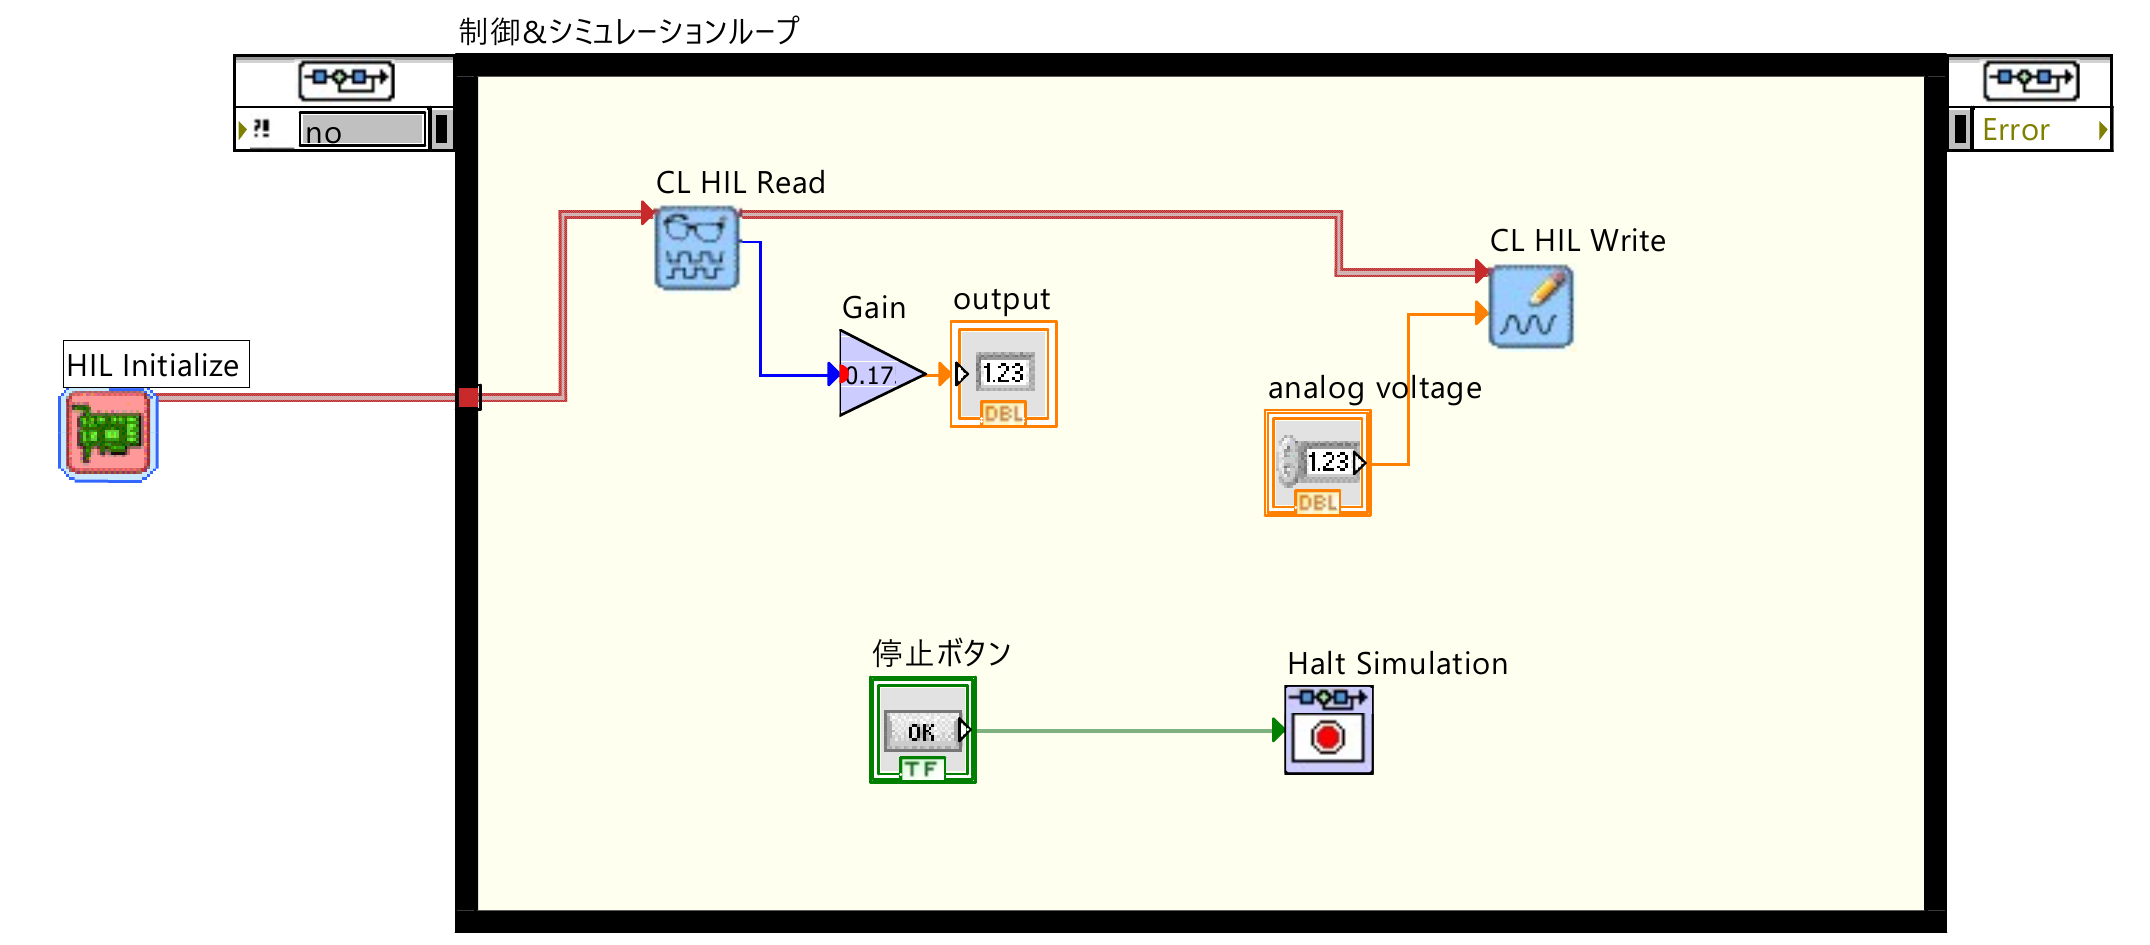
\includegraphics[width=.95\textwidth]{results_figures/exp1_block.png}
 \caption{QUBE Integration 実験で作成した VI のブロックダイアグラム}\label{fig:res1block}
\end{figure}
\begin{figure}[H]\centering
 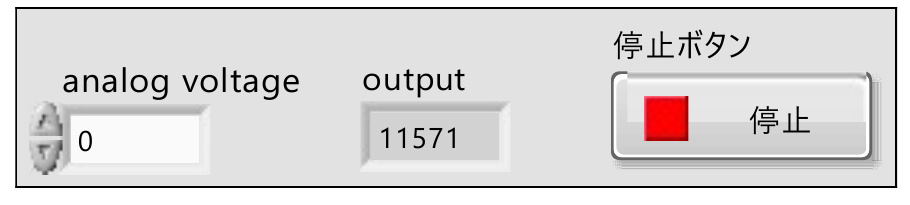
\includegraphics[width=.65\textwidth]{results_figures/exp1_front.png}
 \caption{QUBE Integration 実験のフロントパネル}\label{fig:res1front}
\end{figure}

\subsection{Filtering 実験結果}
エンコーダのカウントをラジアンへ換算し，微分して角速度を表示する VI を図\ref{fig:res2block}に示す。モータ印加電圧は図\ref{fig:res2input}のように約 $1$～$3\,\mathrm{V}$ を往復する方形波であった。フィルタなしおよびカットオフ角周波数を変えた場合の角速度波形を図\ref{fig:res2filter}に示す。いずれの条件でも低電圧区間の定常角速度は約 $22\,\mathrm{rad/s}$，高電圧区間では約 $72\,\mathrm{rad/s}$ と読める。フィルタなしでは定常部分に細かな変動が見られ，$10\,\mathrm{rad/s}$ では平滑な波形になった。$200\,\mathrm{rad/s}$ では高電圧区間の細かな変動が再び見られる。
\begin{figure}[H]\centering
 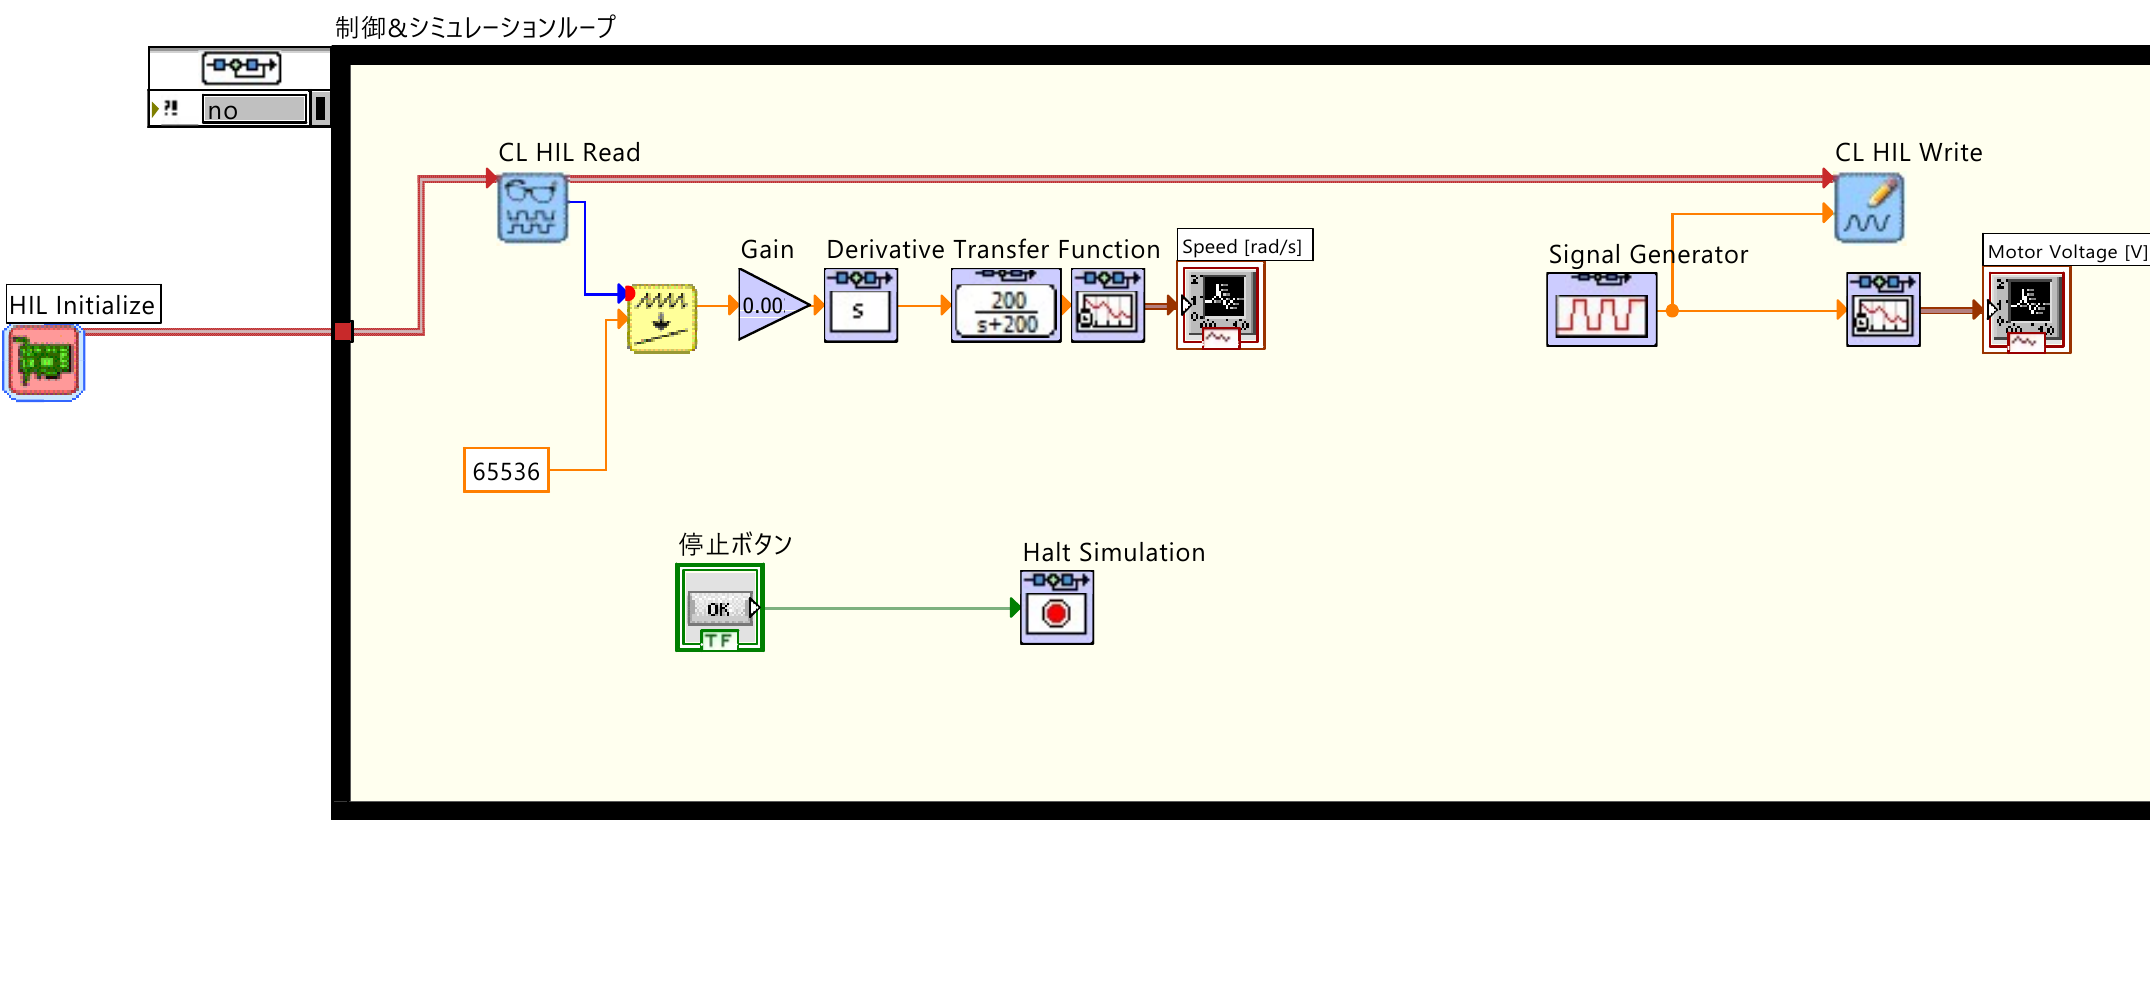
\includegraphics[width=.95\textwidth]{results_figures/exp2_block.png}
 \caption{Filtering 実験で作成した VI のブロックダイアグラム}\label{fig:res2block}
\end{figure}
\begin{figure}[H]\centering
 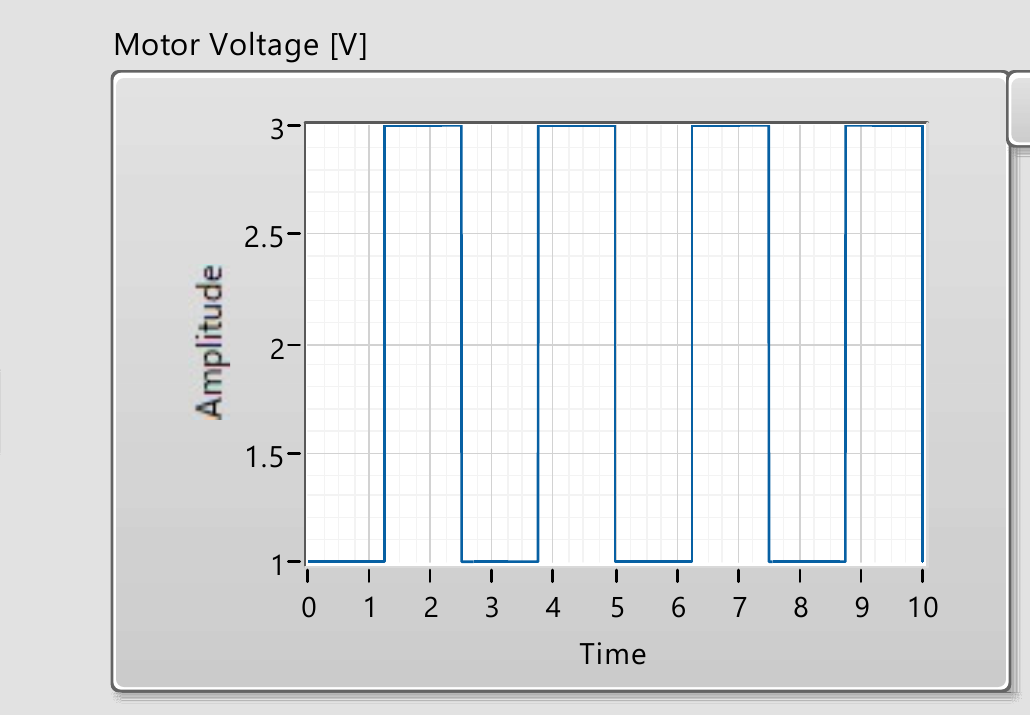
\includegraphics[width=.70\textwidth]{results_figures/exp2_input.png}
 \caption{Filtering 実験時のモータ印加電圧}\label{fig:res2input}
\end{figure}
\begin{figure}[H]\centering
 \begin{minipage}{.48\textwidth}\centering
  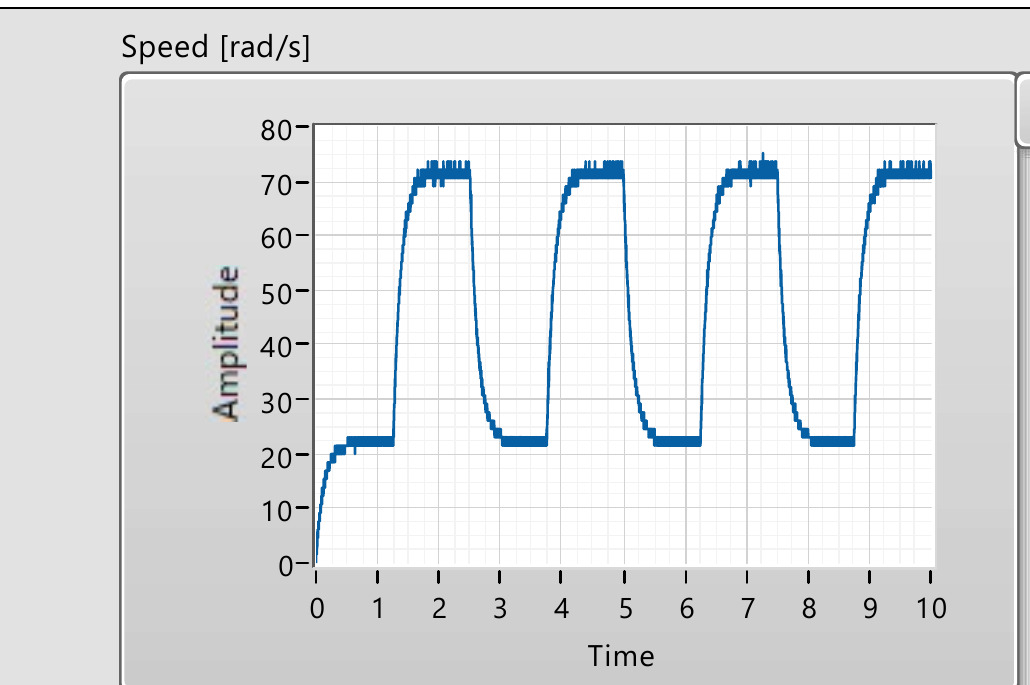
\includegraphics[width=\linewidth]{results_figures/exp2_no_filter.png}\\[-1mm]
  (a) フィルタなし
 \end{minipage}\hfill
 \begin{minipage}{.48\textwidth}\centering
  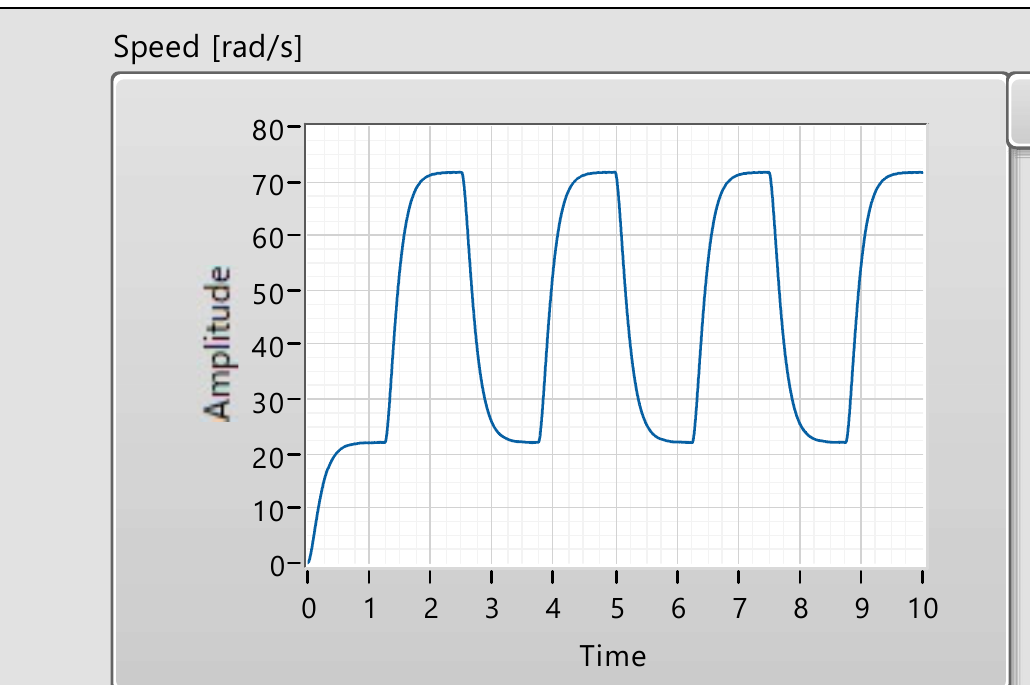
\includegraphics[width=\linewidth]{results_figures/exp2_filter_10.png}\\[-1mm]
  (b) $\omega_f=10\,\mathrm{rad/s}$
 \end{minipage}\\[3mm]
 \begin{minipage}{.48\textwidth}\centering
  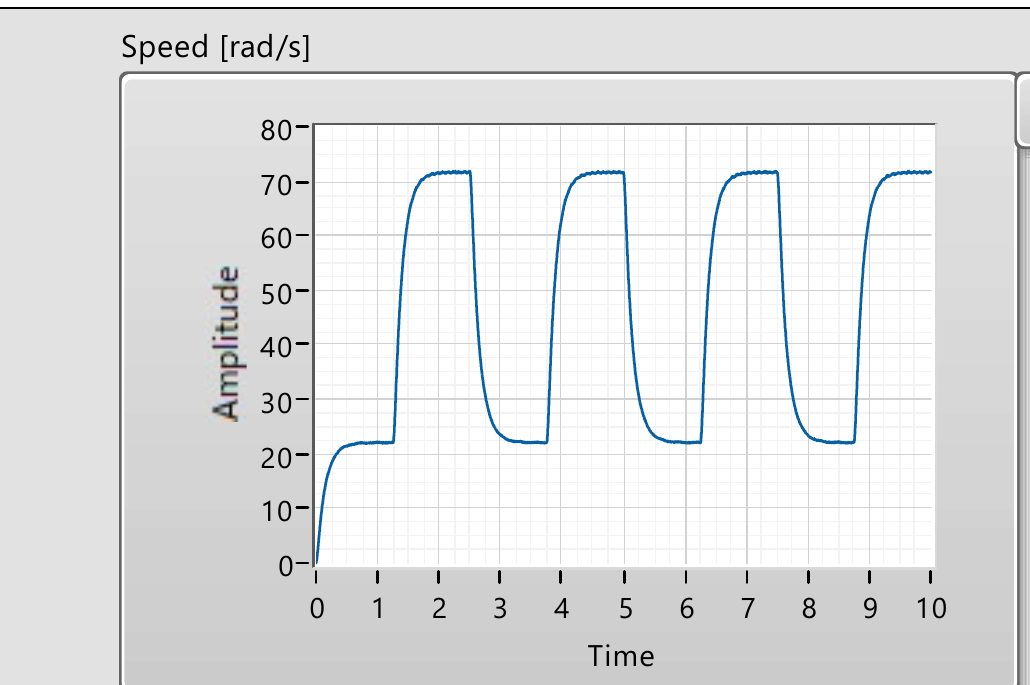
\includegraphics[width=\linewidth]{results_figures/exp2_filter_50.png}\\[-1mm]
  (c) $\omega_f=50\,\mathrm{rad/s}$
 \end{minipage}\hfill
 \begin{minipage}{.48\textwidth}\centering
  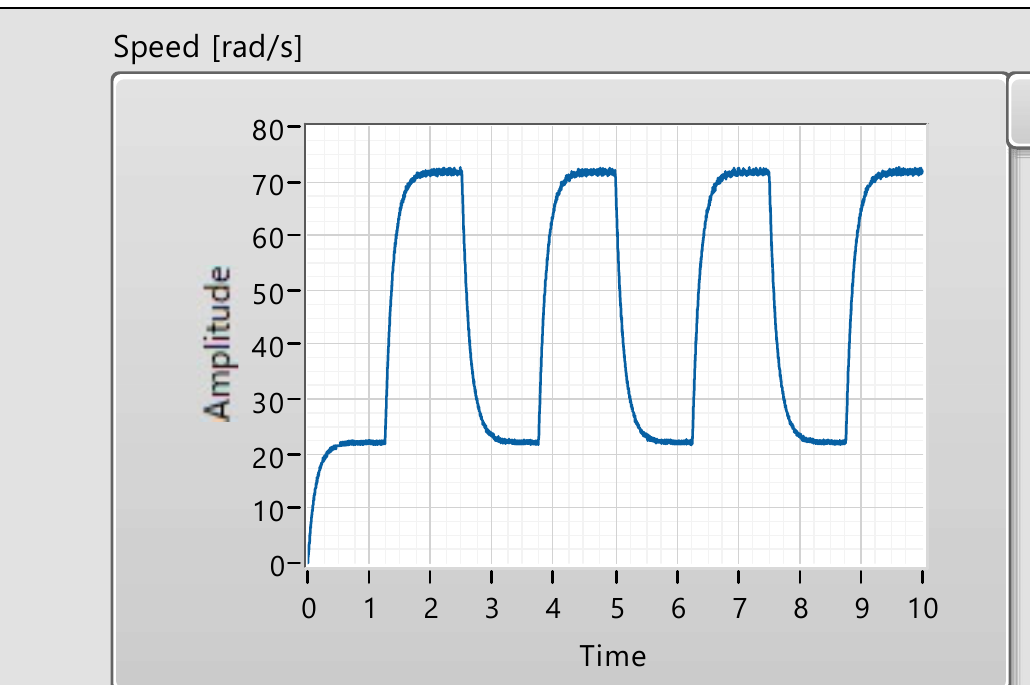
\includegraphics[width=\linewidth]{results_figures/exp2_filter_200.png}\\[-1mm]
  (d) $\omega_f=200\,\mathrm{rad/s}$
 \end{minipage}
 \caption{フィルタ条件による角速度波形の比較。横軸は時間，縦軸は角速度 $[\mathrm{rad/s}]$}\label{fig:res2filter}
\end{figure}
式\eqref{eq:lpf}より，使用したカットオフ角周波数と周波数の対応を表\ref{tab:res2cutoff}に示す。
\begin{table}[H]\centering
 \caption{設定したカットオフ周波数}\label{tab:res2cutoff}
 \begin{tabular}{rr}\toprule
 $\omega_f$ $[\mathrm{rad/s}]$ & $f_f=\omega_f/(2\pi)$ $[\mathrm{Hz}]$\\\midrule
 10 & 1.59\\
 50 & 7.96\\
 200 & 31.83\\\bottomrule
 \end{tabular}
\end{table}

\subsection{Bump Test Modeling 実験結果}
ステップ入力と角速度の取得に用いた VI を図\ref{fig:res3block}に示す。図\ref{fig:res3wave}では，$t\simeq1.0\,\mathrm{s}$ にモータ電圧が $0$ から $2\,\mathrm{V}$ となり，角速度が $0$ 付近から約 $47\,\mathrm{rad/s}$ へ立ち上がっている。XY Graph を図\ref{fig:res3xy}に示す。
\begin{figure}[H]\centering
 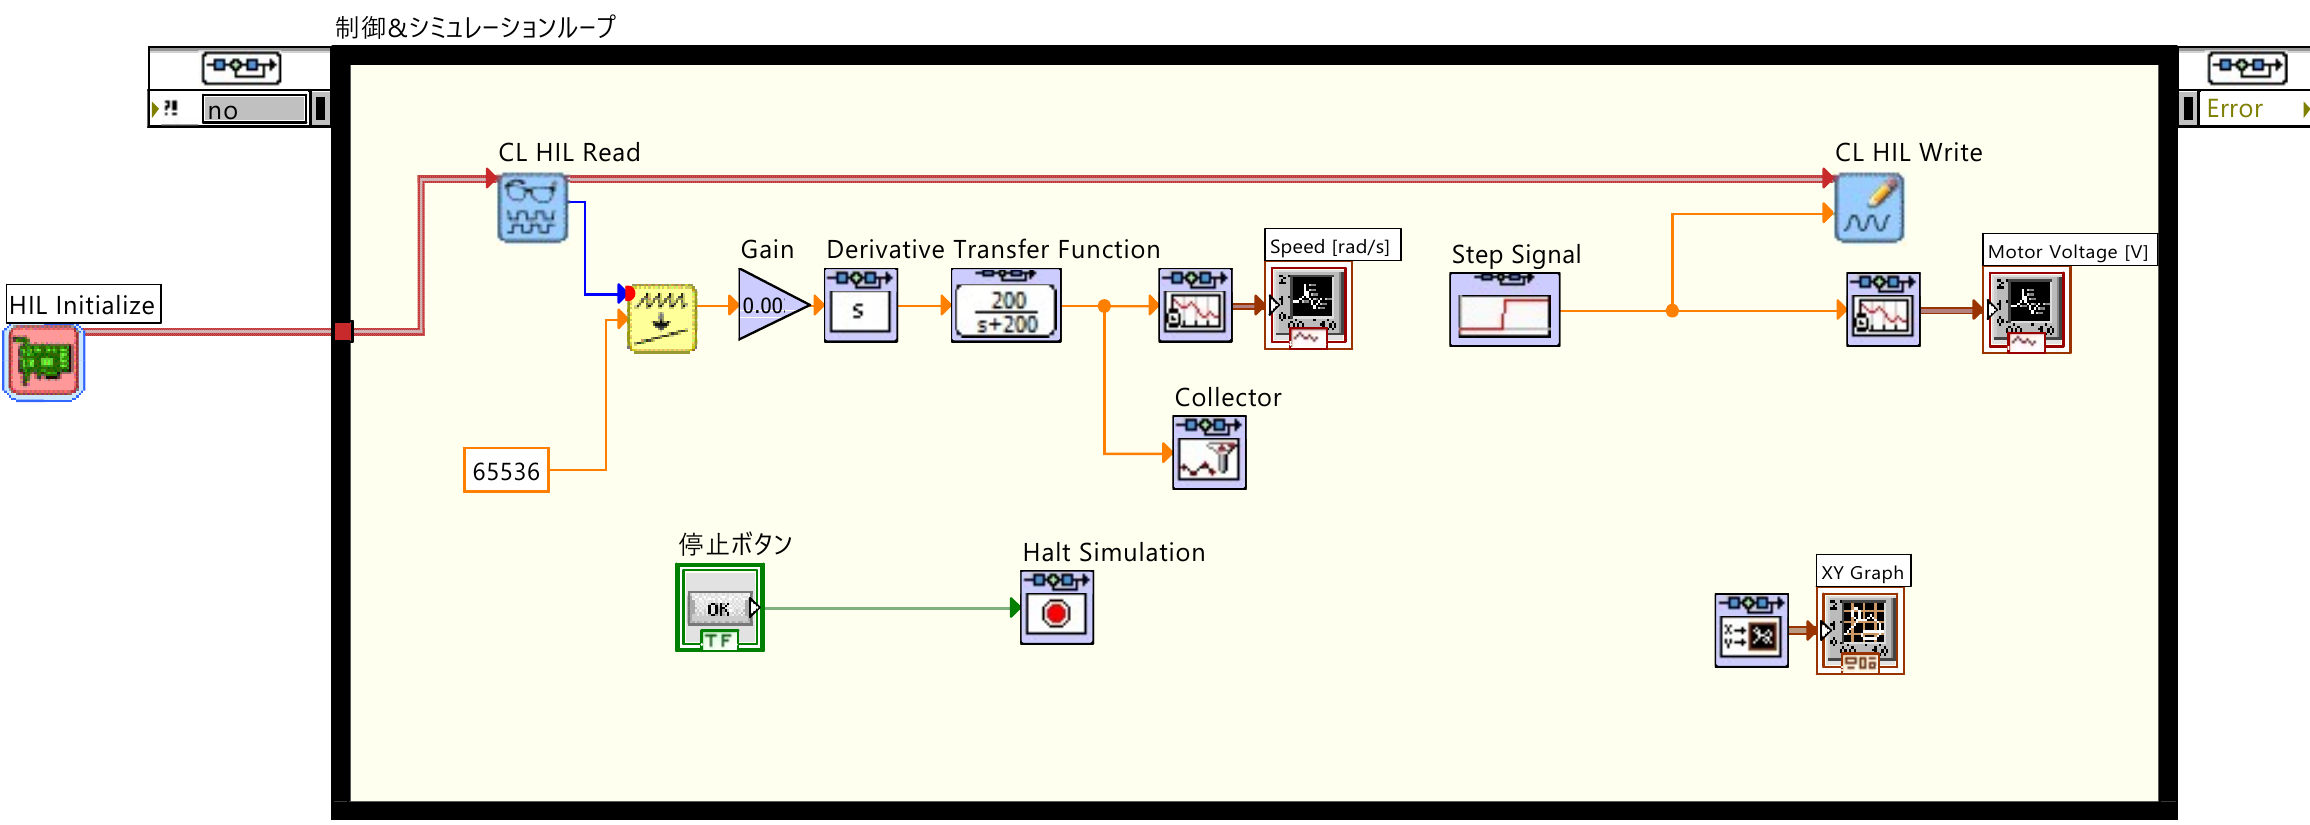
\includegraphics[width=.95\textwidth]{results_figures/exp3_block.png}
 \caption{Bump Test Modeling 実験で作成した VI のブロックダイアグラム}\label{fig:res3block}
\end{figure}
\begin{figure}[H]\centering
 \begin{minipage}{.47\textwidth}\centering
  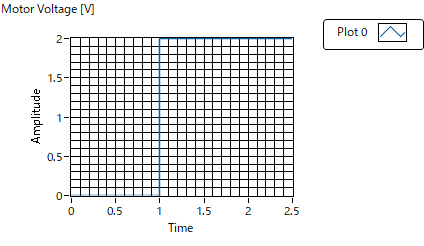
\includegraphics[width=\linewidth]{results_figures/exp3_voltage.png}\\[-1mm]
  (a) モータ印加電圧
 \end{minipage}\hfill
 \begin{minipage}{.47\textwidth}\centering
  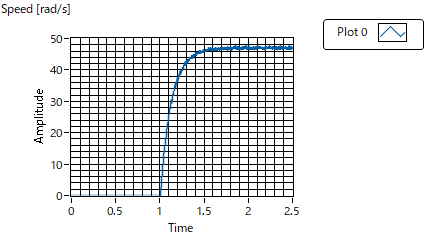
\includegraphics[width=\linewidth]{results_figures/exp3_speed.png}\\[-1mm]
  (b) 測定角速度
 \end{minipage}
 \caption{2 V ステップ入力と角速度応答}\label{fig:res3wave}
\end{figure}
\begin{figure}[H]\centering
 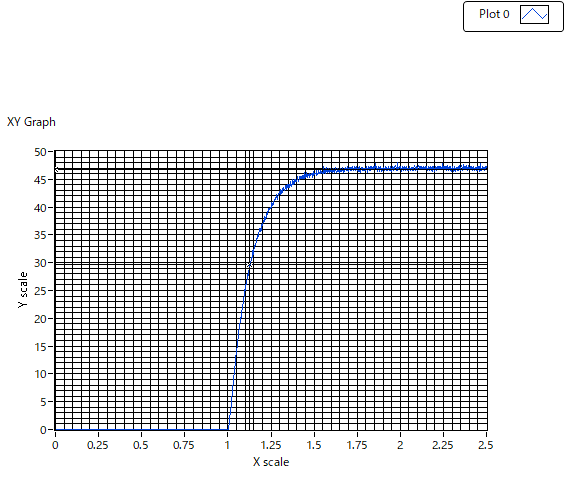
\includegraphics[width=.73\textwidth]{results_figures/exp3_xy.png}
 \caption{バンプテストの角速度を表示した XY Graph}\label{fig:res3xy}
\end{figure}
得られたパラメータは $K=23.42\,\mathrm{(rad/s)/V}$，$\tau=0.128\,\mathrm{s}$ である。入力変化量が $2\,\mathrm{V}$ なので，$K\Delta u=46.84\,\mathrm{rad/s}$，この変化量の63.2\%は $29.60\,\mathrm{rad/s}$ となる。ステップ開始を $t_0=1.000\,\mathrm{s}$ とすると，63.2\%到達時刻は $t_1=1.128\,\mathrm{s}$ である。この値を用いた一次遅れモデルは
\begin{equation}
 G_{\mathrm{bump}}(s)=\frac{23.42}{0.128s+1}
 \label{eq:resultbump}
\end{equation}
である。図\ref{fig:res3compare}では，このモデルによる計算波形と実測波形が立ち上がりから定常状態までほぼ重なっている。
\begin{figure}[H]\centering
 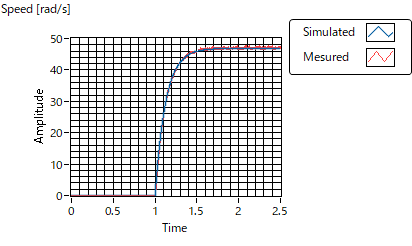
\includegraphics[width=.72\textwidth]{results_figures/exp3_compare.png}
 \caption{バンプテストにおける実測角速度と一次遅れモデルの応答}\label{fig:res3compare}
\end{figure}

\subsection{First Principles Modeling 実験結果}
表\ref{tab:params}に示した慣性ディスクの質量と半径から，ディスクの慣性モーメントは
\begin{equation}
 J_d=\frac{1}{2}m_dr_d^2
 =\frac{1}{2}(0.053)(0.0248)^2
 =1.63\times10^{-5}\,\mathrm{kg\,m^2}
 \label{eq:resultjd}
\end{equation}
となる。したがって，モータ軸まわりの等価慣性モーメントは
\begin{equation}
 J_{\mathrm{eq}}=J_m+J_h+J_d
 =4.0\times10^{-6}+0.6\times10^{-6}+1.63\times10^{-5}
 =2.09\times10^{-5}\,\mathrm{kg\,m^2}
 \label{eq:resultjeq}
\end{equation}
である。この値と式\eqref{eq:current}，式\eqref{eq:motion}を用いて構成した VI を図\ref{fig:res4block}に示す。
\begin{figure}[H]\centering
 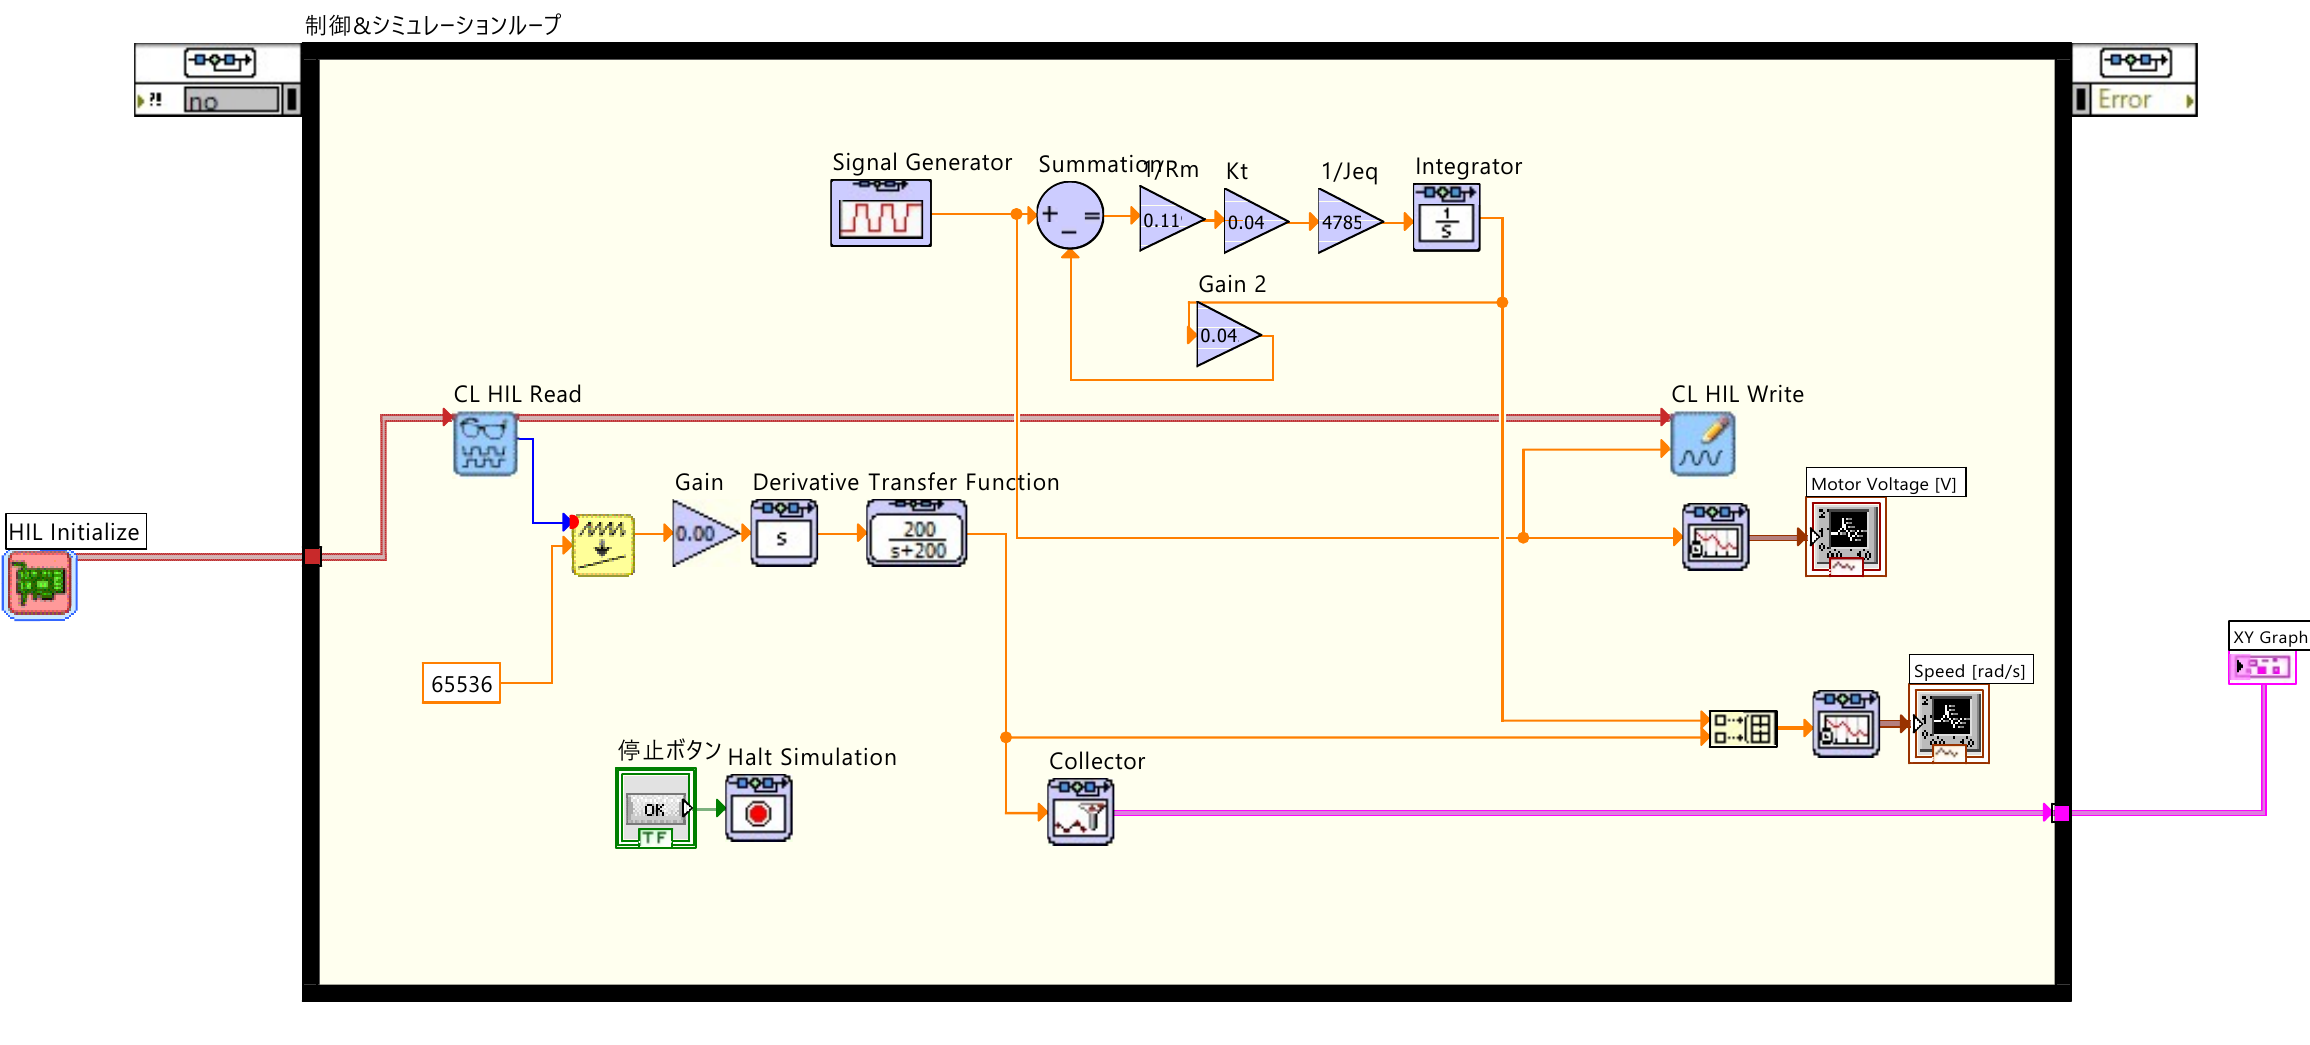
\includegraphics[width=.95\textwidth]{results_figures/exp4_block.png}
 \caption{First Principles Modeling 実験で作成した VI のブロックダイアグラム}\label{fig:res4block}
\end{figure}
図\ref{fig:res4front}に実測角速度とシミュレーション角速度を重ねて示す。印加電圧は約 $1.25\,\mathrm{s}$ で $1$ から $3\,\mathrm{V}$ に切り替わっている。図から読み取った定常角速度は，$1\,\mathrm{V}$ 区間で実測約 $22\,\mathrm{rad/s}$，計算約 $24\,\mathrm{rad/s}$，$3\,\mathrm{V}$ 区間では両者とも約 $72\,\mathrm{rad/s}$ であった。立ち上がりでは計算波形が実測波形より先行している。
\begin{figure}[H]\centering
 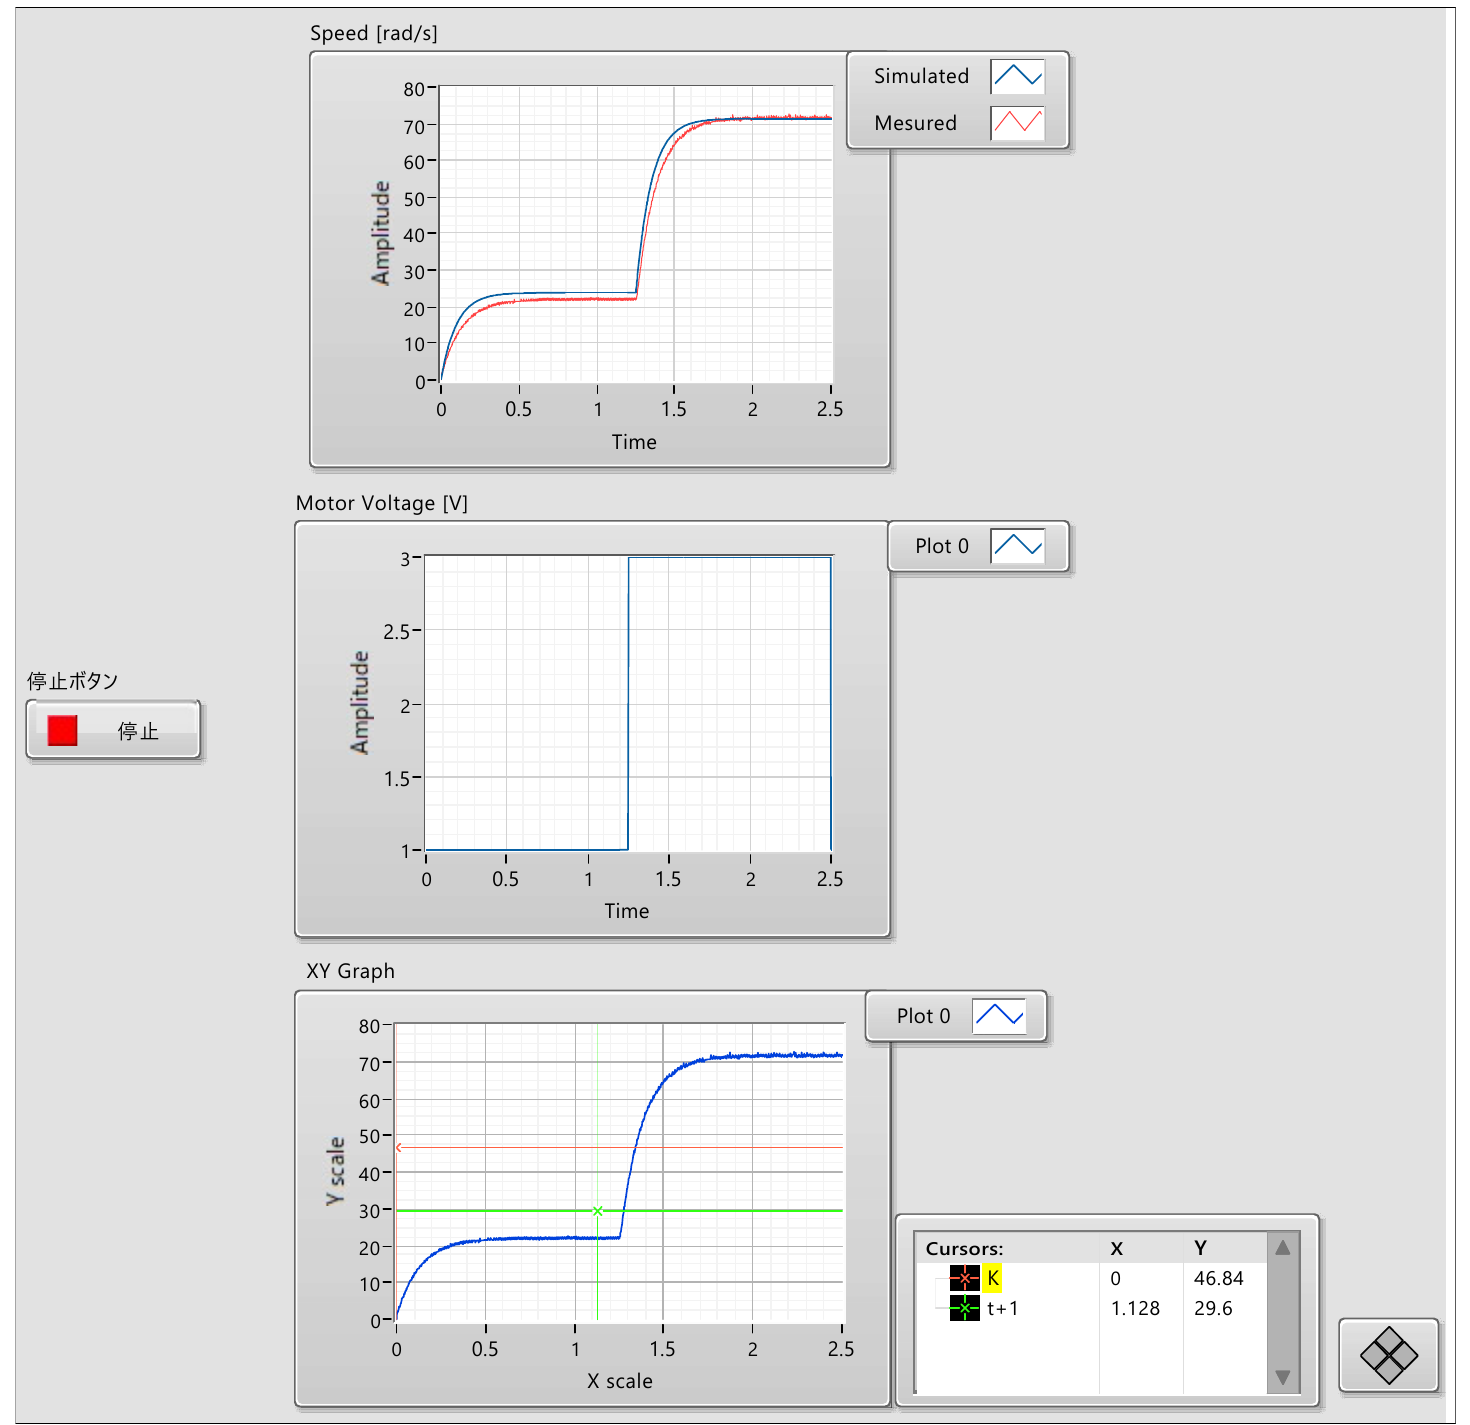
\includegraphics[width=.82\textwidth]{results_figures/exp4_front.png}
 \caption{物理パラメータに基づくモデルと実測角速度の比較（上段），モータ印加電圧（中段），XY Graph（下段）}\label{fig:res4front}
\end{figure}
